\documentclass[a4paper]{article}
\usepackage[spanish,es-tabla]{babel}  %babel es el paquete de idiomas y antes de eso va el o los idiomas que se reuqieren emplear
\usepackage[utf8]{inputenc}
\usepackage{graphicx}
\usepackage{subcaption}
\usepackage[colorlinks=true, citecolor=blue, final]{hyperref}
\usepackage[table]{xcolor}

\setlength{\arrayrulewidth}{1mm}
\setlength{\tabcolsep}{18pt}
\renewcommand{\arraystretch}{2.5}


\usepackage{url} % UTILIZA EL PAQUETE PARA QUE APAREZCA EL URL AUNQUE AUN NOSE SI DEBO ACTIVARLO TAMBIEN EN REFERENCIAS
\hypersetup{
    colorlinks=true,
    linkcolor=blue,
    filecolor=blue,      
    urlcolor=blue,
}
\usepackage{graphicx}
\usepackage[sort&compress, numbers]{natbib}
\usepackage{xcolor}
\usepackage{listings}
\usepackage{ragged2e}
\definecolor{codegreen}{rgb}{0,0.6,0}
\definecolor{codegray}{rgb}{0.5,0.5,0.5}
\definecolor{codepurple}{rgb}{0.58,1,0.82}
\definecolor{backcolour}{rgb}{1,1,0.97}
\lstdefinestyle{mystyle}{
    backgroundcolor=\color{backcolour},   
    commentstyle=\color{codegreen},
    keywordstyle=\color{magenta},
    numberstyle=\tiny\color{codegray},
    stringstyle=\color{codepurple},
    basicstyle=\ttfamily\footnotesize,
    breakatwhitespace=false,         
    breaklines=true,                 
    captionpos=b,                    
    keepspaces=true,                 
    numbers=left,                    
    numbersep=5pt,                  
    showspaces=false,                
    showstringspaces=false,
    showtabs=false,                  
    tabsize=2
}
\lstset{style=mystyle}


\begin{document}  %se utiliza para comenzar lo señalado en el parentesis
\begin{center} %begin para comenzar  agregamos centrar para poner en medio
\large \bf Práctica Nº 4   %\large aumenta ligeramente el texto posterior o alarga 
\\ %\\ Indica brincar espacio. \bf indicara subrayar en negritas las letras despues antes de el termino checar que este en minusculas aveces no entra no se porque pasa un espacio antes y despues de agregar
Diagramas de Voronoi
\end{center} %end terminacion de lo señalado en corchetes en este caso el centrado
\textbf{Nombre:}   %\Textbf marca en negritas la frase entre los corchetes
José Adrián García Fuentes
\hfill  %hfill genera un espacio horizontal para expandirse a lo largo del documento
\textbf{Profesor:}   %para que entre el textbf checar que este todo en minusculas
Satu Elisa Schaeffer \hfill
\\
\textbf{Fecha:} 05/Marzo/2021        %\today agrega la fecha en formato de mes dia, año en ingles agregar un usepackage al principio entre llaves el idioma a emplear y entre corchetes babel que es el paquete de idiomas
\\
\hrule    %hrule agrega una linea horizontal en el documento
\medskip
   %bigskip hace espacio grande entre parrafos medskyp tamaño medio y small skyp uno pequeño  si solo pasas espacios no se despega de una linea y marca error
 \section{Introducción}
\justify Los diagramas de Voronoi son un método comúnmente utilizado para realizar interpolaciones simples. Esta práctica aborda la simulación del crecimiento de un número determinado de semillas sobre una matriz. El material se encuentra dividido en regiones conocidas como celdas de Voronoi que se asemejan a núcleos formados por un proceso de cristalización del material. Si representamos el material con una cuadrícula bidimensional, una celda de Voronoi está formada por las casillas más próximas a cada una de las \textit{k} semillas inicialmente dadas \cite{1}. Una grieta o fractura comienza en las orillas de la cuadrícula y tiene mayor probabilidad de propagarse por las fronteras de las celdas de Voronoi que por el interior de las mismas. Se desea estudiar el efecto que tiene el número de semillas y el tamaño de la zona  \cite{p3}.
\section{Objetivo}  %\section da enfasis a empezar una nueva seccion o tema
\begin{itemize}   %begin comenzar itemize es una viñeta se marca como item no es necesario agregar espacio despues de cada item
    \item Examinar de manera sistemática el efecto del número de semillas y del tamaño de la zona en la distribución de las grietas que se forman en términos de la mayor distancia manhattan entre la grieta y el exterior de la pieza \cite{p3}.

\end{itemize}

%\\ Indica brincar espacio.
\section{Metodología}
\justify
La metodología empleada se realizó a través de RStudio \cite{RStudio} llevando a cabo los pasos señalados en la \textit{Práctica 4: Diagramas de Voronoi} \cite{p3}, se examina las diferencias del número de semillas y del tamaño de la zona en la distribución de las grietas que se forman en terminos de la mayor distancia manhattan entre la grieta y el exterior de la pieza, el código completo de la metodología empleada se encuentra en el repositorio de GitHub \cite{gitadrian}.


\section{Resultados}
\justify
Se obtuvo el código secuencia de GitHub de Schaeffer E. \cite{p3gitdr} y se adecuaron algunas modificaciones variando el número de semillas (10, 20, 40, 60, 80 y 100) y el tamaño de la zona (40, 50, 60, 70, 80, 100) con la finalidad de determinar el efecto que se tiene cambiando el numero de semillas en diferentes tamaños de zonas, se determino el largo de la grieta producida en términos de distancia manhattan determinando que tan lejos llega la grieta del borde, el mínimo de los máximos de la distancia medida de la penetración para evaluar que tan drástica es la fracturación. A continuación se muestra parte del código del experimento \cite{gitadrian} en el cual se señala el número de semillas y tamaño de zona, los datos obtenidos de distancia manhattan fueron agrupados en diagramas tipo violín.
\medskip
\begin{lstlisting}
n <-  c(40, 50, 60, 70, 80, 100)
zona <- matrix(rep(0, n * n), nrow = n, ncol = n)
k <- c(10, 20, 40, 60, 80, 100)
x <- rep(0, k)
y <- rep(0, k) 
for (semilla in 1:k) {
  while (TRUE) { 
    fila <- sample(1:n, 1)
    columna <- sample(1:n, 1)
    if (zona[fila, columna] == 0) {
      zona[fila, columna] = semilla
      x[semilla] <- columna
      y[semilla] <- fila
      break
    }
  }
}
celda <-  function(pos) {
  fila <- floor((pos - 1) / n) + 1
  columna <- ((pos - 1) %% n) + 1
  if (zona[fila, columna] > 0) { # es una semilla
    return(zona[fila, columna])
  } else {
    cercano <- NULL # sin valor por el momento
    menor <- n * sqrt(2) # mayor posible para comenzar la busqueda
    for (semilla in 1:k) {
      dx <- columna - x[semilla]
      dy <- fila - y[semilla]
      dist <- sqrt(dx^2 + dy^2)
      if (dist < menor) {
        cercano <- semilla
        menor <- dist
      }
    }
    return(cercano)
  }
}
\end{lstlisting}
\justify Para cada combinación se obtuvieron las semillas base (figura \ref{b50}), las celdas de Voronoi (figura \ref{b75}) y replicas de las fracturas (figura \ref{b100}), observe la figura \ref{fig:1}.
\medskip
\begin{figure}[h!]
    \centering
\begin{subfigure}[b]{0.3\linewidth}
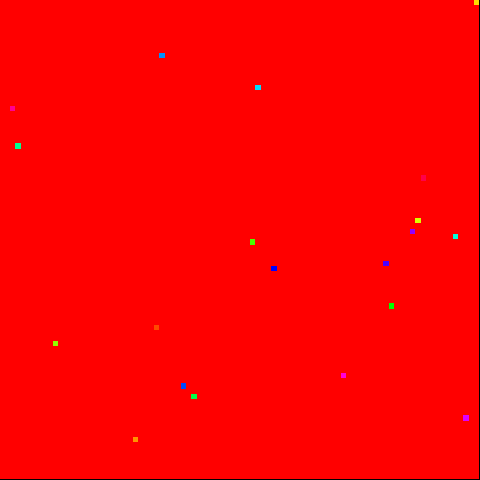
\includegraphics[width=\linewidth]{p4s.png}
\caption{Semillas.}
\label{b50}
\end{subfigure}
\begin{subfigure}[b]{0.3\linewidth}
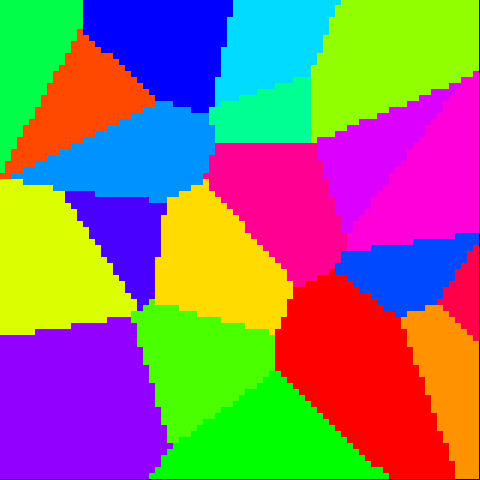
\includegraphics[width=\linewidth]{p4c.png}
\caption{Tamaño $40\times 40$.}
\label{b75}
\end{subfigure}
\begin{subfigure}[b]{0.3\linewidth}
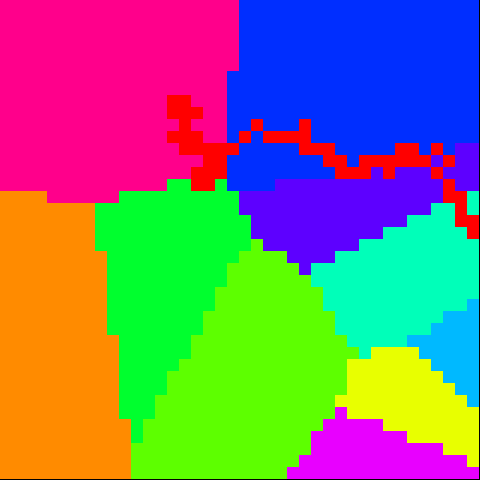
\includegraphics[width=\linewidth]{p410semillas_173.png}
\caption{Fractura.}
\label{b100}
\end{subfigure}
    \caption{Zona de $40\times 40$ con 10 semillas.}
    \label{fig:1}
\end{figure}

\justify En la figura \ref{fig:2} se muestra un número de semillas (figura \ref{b40}) alto en una zona de $40\times 40$ (figura \ref{b41}) se observa que la propagación de la fractura (figura \ref{b101}) es amplia, con el fin de cumplir los propósitos de esta práctica se tomará en cuenta el largo de la grieta en función de que tan lejos llegó desde el borde, en otras palabras tomando en cuenta la medida de penetración de la grieta y el borde para saber que tan drástica es la fracturación. 

\medskip
\begin{figure}[h!]
    \centering
\begin{subfigure}[b]{0.3\linewidth}
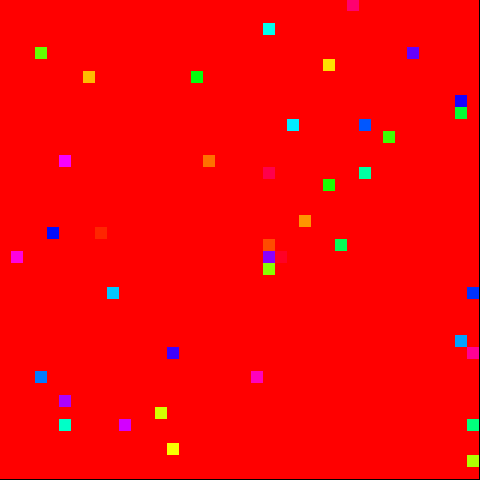
\includegraphics[width=\linewidth]{40semillaszona40.png}
\caption{Semillas.}
\label{b40}
\end{subfigure}
\begin{subfigure}[b]{0.3\linewidth}
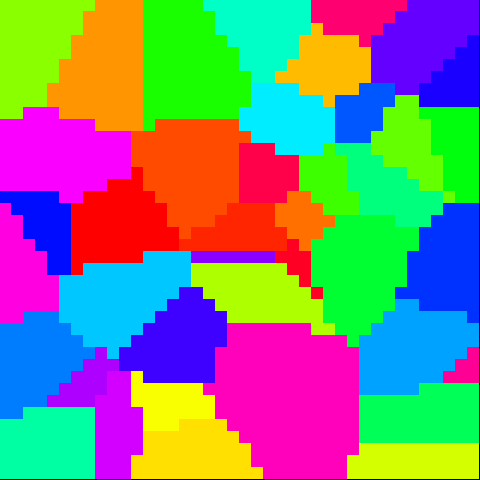
\includegraphics[width=\linewidth]{40 semillas zona40...png}
\caption{Tamaño $40\times 40$.}
\label{b41}
\end{subfigure}
\begin{subfigure}[b]{0.3\linewidth}
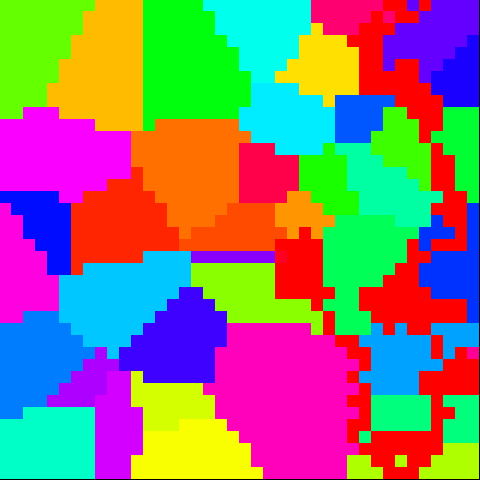
\includegraphics[width=\linewidth]{p440semillas_66.png}
\caption{Fractura.}
\label{b101}
\end{subfigure}
    \caption{Zona de $40\times 40$ con 40 semillas.}
    \label{fig:2}
\end{figure}




\justify Al variar  el número de semillas (figura \ref{b1}) en un determinado tamaño de zonas (figura \ref{b2}) se determinó el efecto de la penetración de la fractura (figura \ref{b3}) en la figura \ref{fig:3} se muestra una zona de $100\times 100$ con un número de semillas bajo, debido aque la probabilidad de que la fractura propague sobre la frontera y no entre los diagramas de Voronoi se obtiene una frecuencia menor de fractura en una zona más grande para un número de semillas más limitado.
\medskip
\begin{figure}[h!]
    \centering
\begin{subfigure}[b]{0.3\linewidth}
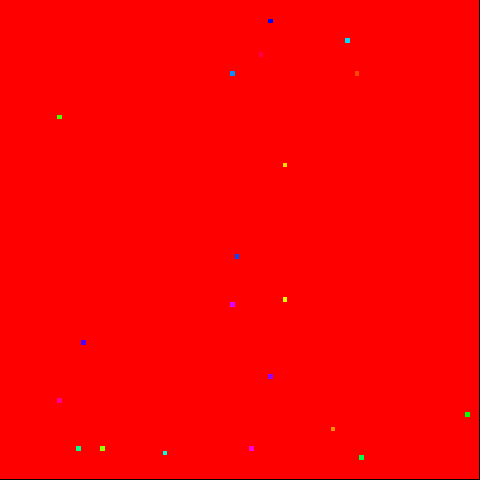
\includegraphics[width=\linewidth]{semillas20z100.png}
\caption{Semillas.}
\label{b1}
\end{subfigure}
\begin{subfigure}[b]{0.3\linewidth}
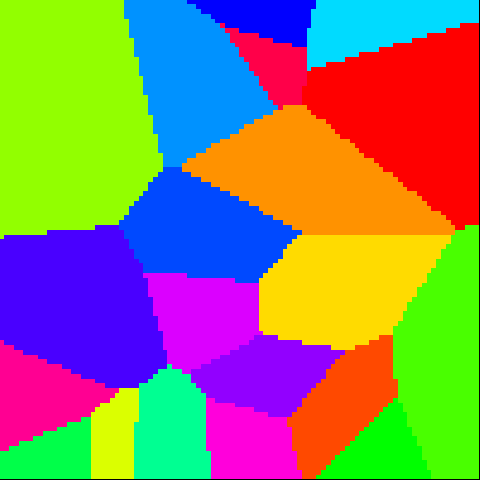
\includegraphics[width=\linewidth]{semillas20zona100.png}
\caption{Tamaño $100\times 100$.}
\label{b2}
\end{subfigure}
\begin{subfigure}[b]{0.3\linewidth}
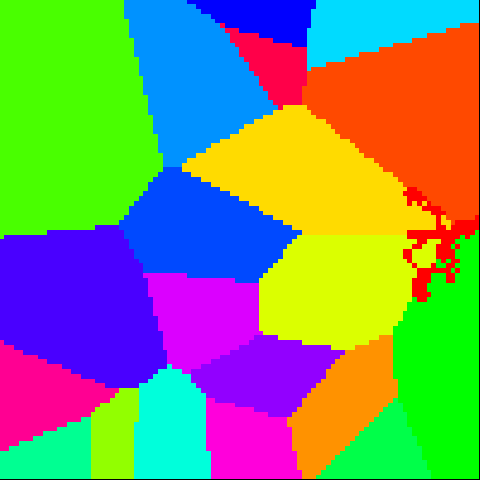
\includegraphics[width=\linewidth]{p420semillas_118.png}
\caption{Fractura.}
\label{b3}
\end{subfigure}
    \caption{Zona de $100\times 100$  con 20 semillas}
    \label{fig:3}
\end{figure}

\justify En la fig \ref{fig:4} y fig \ref{fig:5} se muestra un diagrama de tipo violín que marca la longitud de distancia tipo manhattan variando el tamaño de zona (\textit{n}) en el eje Y, mientras que en el eje X la distancia que penetró la grieta desde el borde tomando en cuenta lo visto en la práctica 1. 

\begin{figure}[h!]
    \centering
\begin{subfigure}[b]{0.45\linewidth}
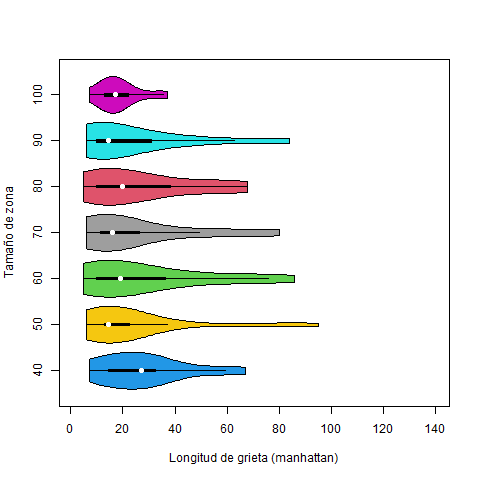
\includegraphics[width=\linewidth]{p4_semillas20.png}
\caption{20 Semillas.}
\label{c1}
\end{subfigure}
\begin{subfigure}[b]{0.45\linewidth}
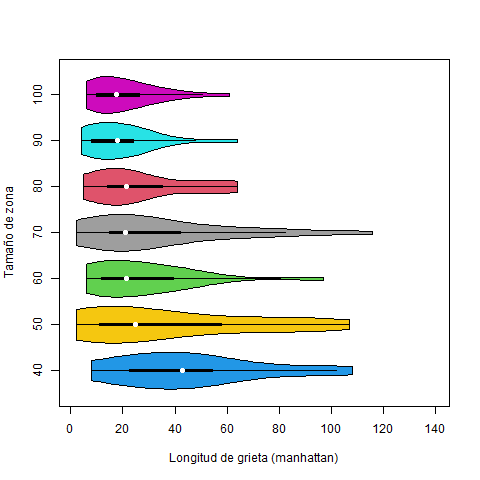
\includegraphics[width=\linewidth]{p4_semillas40.png}
\caption{40 Semillas.}
\label{c2}
\end{subfigure}
\caption{Diagrama de violín con variación en el número de semillas.}
    \label{fig:4}
\end{figure}



\begin{figure}[h!]
    \centering
\begin{subfigure}[b]{0.45\linewidth}
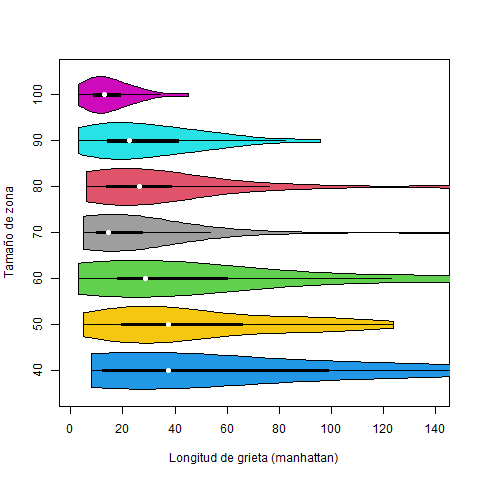
\includegraphics[width=\linewidth]{p4_semillas60.png}
\caption{60 Semillas.}
\label{c4}
\end{subfigure}
\begin{subfigure}[b]{0.45\linewidth}
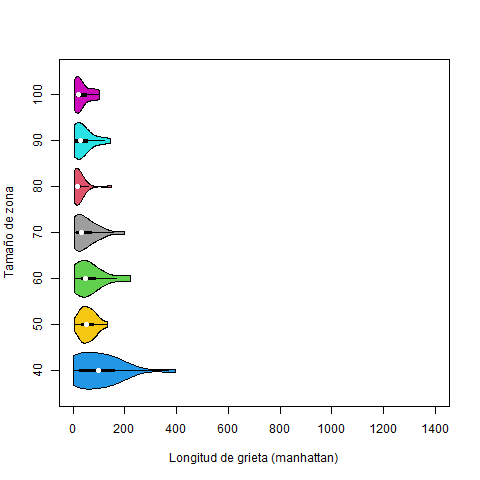
\includegraphics[width=\linewidth]{p4_semillas80.png}
\caption{80 Semillas.}
\label{c5}
\end{subfigure}
\caption{Diagrama de violín con variación en el número de semillas.}
    \label{fig:5}
\end{figure}

\justify Al observar los diagramas se deduce que la densidad de semillas afecta en el comportamiento de la fractura y la distancia que se recorrió como máximo desde el borde al punto de mayor penetración. Para mayor comprensión de lo que pasa en cada experimento se obtuvo archivos .gif donde se muestra distintos recorridos de la fractura, los gráficos de las distancias manhatan para 10 y 100 semillas se encuentran en el repositorio de GitHub \cite{gitadrian}.
\medskip
\justify En el cuadro \ref{fig:1} se muestra un fragmento \cite{gitadrian} de las distancias máximas alcanzadas desde el borde hasta lo máximo que penetro del eje la fractura.

\centering
{\rowcolors{3}{blue!90!yellow!10}{blue!80!yellow!5}
\begin{tabular}{ |p{3cm}|p{1cm}|p{1cm}|  }
\hline
\multicolumn{3}{|c|}{Distancia Manhattan} \\
\hline
\label{m}
\caption{Distancias Manhattan}
Zona. & Semillas. & Distancia desde borde \\
\hline
Tamaño $40\times 40$. & $10 & $18 \\
Tamaño $50\times 50$. & $20   & $26 \\
Tamaño $60\times 60$. & $40 & $50 \\
Tamaño $70\times 70$.& $60 & $48 \\
Tamaño $80\times 80$.& $80 & $66 \\
Tamaño $100\times 100$.& $100 & $83 \\
\hline
\end{tabular}
}
\medskip
\justify
\section{Conclusión}
\justify Al examinar el efecto del número de semillas y del tamaño de la zona en la distribución de las grietas que se forman en términos de la mayor distancia manhattan entre la grieta y el exterior de la pieza se observa que a un mayor número de semillas y una dimensión reducida la grieta propagara un mayor número de veces, aunque la grieta del mismo modo en una dimensión más grande puede propagar con mayor facilidad el número de veces que propaga es menor debido a la frontera entre semillas, es importante mencionar que si el número de semillas es bajo en una zona muy grande la posibilidad de generar una fractura sera demasiado baja tomando como ejemplo la metodología de 10 semillas en una zona de 100 x 100.   

\bibliography{practica4} %\bibliography dentro de los corchetes aparece el comando seccion de referencias  sin embargo para que aparezca tiene que aparecer la seccion \bibliographystyle para dar un estilo del tipo de letra o tipo de acomodo que llevara 
\bibliographystyle{ieeetr}   %\da un estilo de acomodo dependiendo del comando dentro d corchetes
\end{document} %indica finalizacion de lo señalado en el parentesis en este caso el documento

